% Reporte técnico final completo, para revisión interna. Mismo texto que los archivos de secciones.
% Se genera a partir de secciones/*.md y refs_cuerpo.tex. Compilar con: xelatex reporte_completo.tex (dos veces).
\documentclass[11pt,letterpaper]{article}
\usepackage[margin=2.54cm]{geometry}
\usepackage{fontspec}
\setmainfont{TeX Gyre Termes}
\usepackage{polyglossia}
\setdefaultlanguage{spanish}
\usepackage{graphicx}
\usepackage{url}
\urlstyle{same}
\usepackage{enumitem}
\usepackage{fancyhdr}
\setlength{\headheight}{14pt}
\setlength{\emergencystretch}{3em}
\setlength{\parskip}{6pt}
\setlength{\parindent}{0pt}
\newcommand{\bibref}[1]{\par\noindent\hangindent=1.27cm\hangafter=1 #1\par\vspace{0.6em}}
\usepackage{titlesec}
\titleformat{\section}{\large\bfseries}{\thesection.}{0.5em}{}
\begin{document}
\begin{titlepage}
\centering

\includegraphics[height=2.2cm]{figuras/logo_buap.png}\hfill
\includegraphics[height=2.2cm]{figuras/logo_fcc.png}\par
\vspace{1.2cm}
{\large Benemérita Universidad Autónoma de Puebla\par Facultad de Ciencias de la Computación\par}
\vspace{2cm}
{\LARGE\bfseries Reporte técnico final\par}
\vspace{0.6cm}
{\Large Reto AgroCebada FIRA 2026\par}
\vspace{0.4cm}
{\large Estimación del rendimiento de cebada de temporal y su uso en la inclusión financiera\par}
\vspace{2cm}
{\large\bfseries Equipo Los Bien Dotados\par}
\vspace{0.5cm}
José Alán Pomares Valdés\par
Vicente Josimar López Martínez\par
Luis Emmanuel Ramiro Luna\par
\vspace{0.8cm}
{\bfseries Asesor}\par
Luis Gustavo Olivares Soto\par
\vfill
Puebla, México, 15 de octubre de 2026\par
\end{titlepage}
\pagestyle{fancy}
\fancyhf{}
\fancyhead[L]{Los Bien Dotados}
\fancyhead[R]{Reto AgroCebada FIRA 2026}
\fancyfoot[C]{\thepage}
\setlength{\parskip}{6pt}
\section{Introducción}

El Reto AgroCebada FIRA 2026 pide estimar el rendimiento de grano de cebada de temporal, en toneladas por hectárea (t/ha), de 59 parcelas (Fideicomisos Instituidos en Relación con la Agricultura [FIRA], 2026a). El conjunto de datos reúne 197 parcelas del ciclo primavera-verano 2025, de abril a octubre, en nueve municipios de Puebla, Hidalgo y Tlaxcala. De ellas, 138 traen su rendimiento y sirven para entrenar, y 59 no lo traen y son las que se califican. FIRA hizo la partición al azar, estratificada, con proporción 70 y 30 \%. Las tres entidades se cuentan entre las cuatro principales productoras de cebada grano del país (Secretaría de Agricultura y Desarrollo Rural [SADER], 2025).

El rendimiento es el peso de toda la cosecha medido en báscula, sin ajuste por humedad, impurezas ni mermas. FIRA aclaró en sus sesiones de preguntas que la fuente es mixta, principalmente la comercializadora que compró el grano y, en menor proporción, el productor, y que no informará la fuente de cada parcela (FIRA, 2026b). Por eso tratamos todos los registros como una sola variable objetivo. Las variables explicativas son series de Sentinel-2 (Drusch et al., 2012), Landsat y PlanetScope (Frazier y Hemingway, 2021), lluvia (Funk et al., 2015), temperatura (Verdin et al., 2020) y topografía de INEGI.

La predicción de rendimiento con aprendizaje automático y teledetección es un tema muy estudiado, como lo resumen van Klompenburg et al. (2020) y Weiss et al. (2020). La literatura también reporta que el rendimiento declarado contiene un error considerable (Lobell et al., 2020). En este reto la muestra es pequeña y el registro del rendimiento no es homogéneo. Por ello, además de preguntar qué algoritmo predice mejor, preguntamos qué información predice de verdad el rendimiento y qué tan confiable es el error que estimamos.

Nuestro primer hallazgo fue sobre las etiquetas, pues cada municipio registra el rendimiento de una de dos formas. En cuatro municipios los valores tienen dos decimales y promedian 4.49 t/ha, y en los otros cinco están redondeados a 0.5 o a 0.1 t/ha y promedian 3.05 t/ha. Llamamos a estas formas régimen A y régimen B. Es una observación. La fuente mixta es una explicación posible que no podemos confirmar.

Con esa base seguimos un proceso explícito. Antes de probar ideas fijamos cómo las evaluaríamos. Después agregamos las piezas del modelo una por una y conservamos solo las que reducían la raíz del error cuadrático medio (RMSE) en validación y superaban una prueba de permutación. El RMSE se expresa en t/ha y castiga más los errores grandes. También reportamos el error absoluto medio (MAE) y el coeficiente de determinación (R²), que es la fracción de la variación del rendimiento que explica el modelo.

El modelo final es un proceso gaussiano que usa el régimen de registro del municipio y el rendimiento de las parcelas vecinas del mismo régimen que están a 400 m o menos. No usa imágenes de satélite ni clima, porque ninguno mejoró la validación. Su error esperado es de 0.46 a 0.49 t/ha y mejora poco a la media por régimen.

Además del modelo, desarrollamos una capa que traduce la predicción a pesos y a riesgo de crédito, y una aplicación web para consultarla.

\section{Justificación}

FIRA canaliza financiamiento al sector agropecuario, y sus decisiones productivas, de planeación y eventualmente financieras requieren estimar cuánto producirá una parcela. En la cebada de temporal el costo por hectárea es alto y la cosecha depende del clima. Una estimación del rendimiento con su incertidumbre ayuda a valorar si la cosecha cubrirá el crédito y el costo de producción.

Los datos de campo son escasos y costosos, mientras que las imágenes de satélite y los datos climáticos son públicos y cubren cualquier parcela. Por eso es útil saber cuánta información del rendimiento contienen esas fuentes y cuánta proviene del propio registro de los productores. Con 138 parcelas de entrenamiento y etiquetas con fuente mixta, también es útil medir con rigor qué tan confiable es el error y no solo reportar el mejor valor observado.

Este trabajo aporta una estimación auditable, con un error calculado de forma conservadora, una traducción a pesos por hectárea y una aplicación web para analistas y productores. También documenta las ideas que no funcionaron, para que trabajos futuros no repitan pruebas sin resultado.

\section{Objetivos}

\textbf{Objetivo general.} Estimar el rendimiento de cebada de temporal, en t/ha, de las 59 parcelas del reto con el menor RMSE posible sobre parcelas no vistas, y reportar con honestidad qué tan confiable es esa estimación y qué información la sustenta.

\textbf{Objetivos específicos.}

\begin{enumerate}

\item Caracterizar las etiquetas de rendimiento y determinar cómo su forma de registro afecta lo que un modelo puede predecir.

\item Construir el modelo agregando una pieza a la vez, con una regla de decisión fijada antes de probar, y conservar solo las piezas que mejoren la validación.

\item Estimar el error esperado con validación anidada y entregar para cada parcela un intervalo de predicción del percentil 10 al 90.

\item Responder con evidencia las tres preguntas guía sobre el índice satelital, la variable climática y la combinación de variables de mayor peso.

\item Traducir el error a pesos por hectárea y a una señal de riesgo de crédito, e indicar en qué momento del ciclo puede usarse la herramienta y con qué información.

\item Entregar una aplicación web que permita consultar las predicciones, sus intervalos y la probabilidad de quedar bajo un umbral elegido por el usuario.

\end{enumerate}

\section{Metodología}

\textbf{Datos y preparación.} Usamos las 197 parcelas y los datos satelitales, climáticos y topográficos del reto. Consideramos limpia una observación con nubosidad de 20 \% o menos y con valor del índice, y descartamos las demás sin imputar. De las series construimos 91 variables por parcela, como el máximo del NDVI de 2025, la fenología (Zadoks et al., 1974), la historia de 2022 a 2024, la heterogeneidad dentro de la parcela, el clima y la topografía. Ninguna usa el rendimiento.

\textbf{Régimen de registro.} Cada municipio registra las etiquetas de una sola forma. Asignamos el régimen con una regla fija por municipio, que no se recalcula en la validación ni usa el rendimiento de la parcela evaluada. En seis parcelas de municipios con una a tres parcelas de entrenamiento el régimen se dedujo de su propia etiqueta. Sin ellas el RMSE pasa de 0.458 a 0.464 t/ha.

\textbf{Evaluación.} Usamos validación cruzada de cinco grupos repetida 10 veces y estratificada por municipio, que imita la partición oficial. Es el esquema A, que decide. El esquema B deja fuera zonas completas, formadas al unir parcelas a menos de 2 km, como recomiendan Roberts et al. (2017) y Ploton et al. (2020), y mide la dependencia de los vecinos. Todo lo que usa el rendimiento se recalcula dentro de cada grupo, para que la parcela evaluada no influya en su propia predicción.

\textbf{Regla de decisión.} Fijamos de antemano que una idea se acepta si baja el RMSE en al menos 7 de las 10 repeticiones y si supera una prueba de permutación (Ojala y Garriga, 2010). En la prueba revolvemos las variables nuevas dentro de cada régimen y repetimos la validación 50 veces. Exigimos un valor p de 0.05 o menos. Registramos 73 evaluaciones sin corregir por comparaciones múltiples, así que los valores p son aproximados.

\textbf{Modelo final.} Es un proceso gaussiano (Rasmussen y Williams, 2006) con núcleo de base radial más un término de ruido. Sus entradas son el régimen y el rezago espacial. El rezago es el promedio, ponderado por el inverso de la distancia, del rendimiento de hasta 10 parcelas de entrenamiento del mismo régimen a 400 m o menos (Tobler, 1970). Sin vecinos, recibe la media de su régimen. Al calcular el rezago de una parcela de entrenamiento la excluimos a ella misma. Los parámetros se ajustan por máxima verosimilitud con las parcelas de entrenamiento.

\textbf{Intervalos.} Usamos predicción conformal dividida de Mondrian, que calibra por separado cada régimen, según Vovk et al. (2005) y Lei et al. (2018). Guardamos los errores con signo de las predicciones fuera de grupo, sumamos a cada predicción los cuantiles 0.10 y 0.90 de los errores de su régimen y con ellos estimamos la probabilidad de quedar bajo un umbral.

\textbf{Controles de confiabilidad.} Estimamos el error esperado con validación anidada, que repite la elección entre 12 variantes dentro de cada grupo externo (Varma y Simon, 2006), lo que corrige el sesgo de elegir el mejor entre muchos (Cawley y Talbot, 2010). Comparamos modelos con una prueba t corregida por el traslape de repeticiones (Nadeau y Bengio, 2003). Buscamos fuga de información revolviendo los rendimientos dentro de cada régimen, y una prueba automatizada verifica que alterar las etiquetas de prueba no cambia las predicciones. Para el margen de calificación sorteamos 5000 grupos de 59 errores, 37 del régimen A y 22 del B.

\textbf{Preguntas guía.} Usamos un bosque aleatorio de análisis, distinto del modelo final, y medimos cuánto sube su RMSE al revolver todas las variables de un índice o de un grupo climático. Lo hicimos con y sin el régimen, con cinco repeticiones.

\textbf{Capa económica.} Valuamos la predicción con el precio medio rural del Servicio de Información Agroalimentaria y Pesquera (SIAP, 2026) de 2023 a 2025 y con los costos del paquete de FIRA de primavera-verano 2022 (FIRA, s. f.), actualizados a 2025 con el índice general de precios de INEGI. Calculamos los puntos de equilibrio y la probabilidad de no cubrirlos con los errores del modelo y la pérdida histórica del municipio.

\textbf{Modelo municipal.} Como complemento, ajustamos un modelo con el rendimiento municipal del SIAP de 2003 a 2025.

\section{Resultados y discusión}

\textbf{Error del modelo.} En validación cruzada repetida el modelo obtiene un RMSE de 0.458 t/ha, un MAE de 0.312 t/ha y un R² de 0.71. La media por régimen, que no usa vecinos, obtiene 0.489. El RMSE del modelo menos el de la media por régimen es −0.029 t/ha, con un intervalo de confianza del 95 \% de −0.079 a +0.022. El signo negativo favorece al modelo, pero el intervalo incluye el cero y la diferencia no es significativa. Con validación anidada el RMSE del procedimiento completo es 0.490. Por ello esperamos un error de 0.46 a 0.49 t/ha en las 59 parcelas. Con 59 parcelas el RMSE calculado varía además por azar, y el 90 \% de los sorteos cae entre 0.35 y 0.56 t/ha.

\textbf{Qué aportó cada pieza.} El régimen fue la pieza principal. Las medias de los regímenes difieren en 1.4 t/ha, casi tres veces la desviación dentro de cada uno. El rezago espacial bajó el RMSE a 0.470 con un modelo lineal, y el proceso gaussiano a 0.458. Con coordenadas revueltas ninguna de 50 permutaciones igualó el error real (p = 0.02). Las variables satelitales, climáticas y topográficas no mejoraron la validación, y juntar todas las satelitales empeoró el RMSE a 0.498. En el esquema B el modelo empata con la media por régimen (0.489), como se espera sin vecinos cercanos. Las 59 parcelas tienen más vecinos que las de validación (61 \% contra 46 \% con un vecino a 400 m o menos), lo que podría favorecer el extremo bajo, aunque no lo demostramos.

\textbf{Intervalos.} El intervalo del percentil 10 al 90 cubre 0.826 de las parcelas en validación anidada (intervalo de confianza de 0.765 a 0.883), con un ancho medio de 1.13 t/ha. Las predicciones del régimen A promedian 4.49 t/ha y las del B 3.06 t/ha. En 18 parcelas, todas del régimen B, la probabilidad de quedar bajo 2.5 t/ha supera 0.10.

\begin{figure}[ht]
\centering
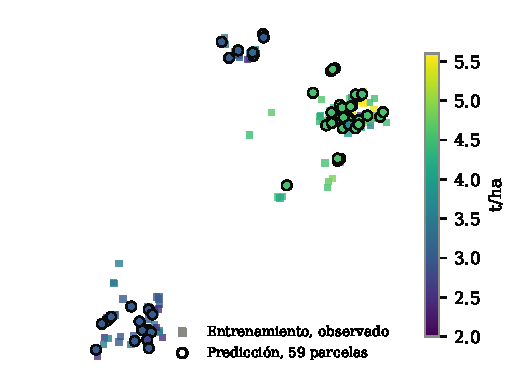
\includegraphics[width=0.78\textwidth]{figuras/f12_mapa.pdf}
\caption{Rendimiento observado en las parcelas de entrenamiento (cuadros) y predicho en las 59 parcelas (círculos con borde), con la misma escala de color. Los grupos en tonos oscuros, al oeste, son del régimen B.}
\end{figure}
\begin{figure}[ht]
\centering
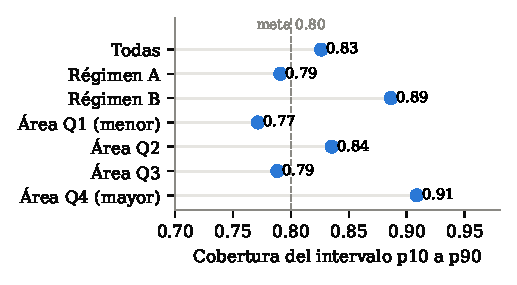
\includegraphics[width=0.78\textwidth]{figuras/f10_cobertura.pdf}
\caption{Fracción de parcelas cuyo rendimiento cae dentro de su intervalo del percentil 10 al 90, por régimen y por cuartil de área. La meta es 0.80.}
\end{figure}

\textbf{Preguntas guía.} Primero, el índice más importante depende del escenario. Sin el régimen, el NDVI es el mayor, pues revolverlo sube el RMSE 0.106 t/ha, pero el NDVI histórico de la parcela identifica la zona y funciona como sustituto del régimen. Con el régimen y el rezago presentes, el índice de sequía NDDI (Gu et al., 2007) es el mayor, con 0.004 t/ha (de 0.002 a 0.006), un efecto muy pequeño. Segundo, la variable climática de mayor peso sin el régimen es la lluvia, con 0.364 t/ha, pero sus celdas de 5 km identifican la zona. Con el régimen presente ninguna aporta. Tercero, la mejor combinación es el régimen más el rezago espacial. Ningún bloque satelital o climático adicional pasó la regla de decisión. Estas importancias salen del bosque de análisis y no del modelo final.

\textbf{Error en términos productivos.} Con el precio medio de 5,353 \$/t en el régimen A y de 5,693 \$/t en el B, un error de 0.46 t/ha equivale a unos 2,500 \$/ha, y a entre 2,000 y 3,300 \$/ha con los precios municipales de 4,291 a 7,224 \$/t. El costo total del paquete es de 24,773 a 28,377 \$/ha, así que el error equivale de 9 a 10 \% del costo. Frente al crédito por hectárea, de 6,561 a 15,015 \$/ha, equivale de 17 a 38 \%. El ancho del intervalo, 1.13 t/ha, equivale a unos 6,000 a 6,400 \$/ha.

\textbf{Limitaciones para una decisión real.} Primero, el RMSE es un promedio, y las parcelas con rendimientos extremos, como las de 5.5 t/ha en Chignahuapan, quedan cerca de la media de su régimen. Segundo, las predicciones están en las unidades de la etiqueta, sin ajuste por humedad ni impurezas, y no equivalen al grano vendible. Tercero, el margen estimado depende más del precio y del costo que del error de rendimiento, pues el precio del SIAP mezcla grano aceptado y rechazado y los costos de 2022 se actualizaron con un índice general. Cuarto, solo hay una temporada, con mayo y junio más lluviosos de lo normal. Quinto, el modelo usa rendimientos de parcelas vecinas de la misma temporada, que existen solo tras su cosecha, así que es una estimación de cierre de temporada.

\textbf{Aplicación web.} Muestra un mapa de las parcelas, la predicción de cada una con su intervalo del percentil 10 al 90 y la probabilidad de quedar bajo un umbral que elige el usuario, y ejecuta el modelo en vivo. Está disponible en \url{https://agrocebada.alan-pv.com}.

\textbf{Limitaciones del análisis.} El modelo apenas mejora a la media por régimen. El régimen es una observación por municipio, y la fuente mixta es una explicación posible sin confirmar. No medimos el ruido de etiqueta. Si el redondeo del régimen B fuera uniforme, por sí solo aportaría unos 0.13 t/ha de error en ese régimen. Es una cota aproximada, no un límite demostrado.

\section{Uso de la ciencia de datos en la inclusión financiera del sector agro}

El acceso del productor a crédito depende de que quien presta pueda valorar el riesgo de su cosecha. La ciencia de datos sustituye un rendimiento supuesto por una estimación de cada parcela con su incertidumbre.

\textbf{Capa de crédito.} Calculamos por parcela el rendimiento que cubre el crédito y el que cubre el costo total, y la probabilidad de no alcanzarlo. La probabilidad combina los errores del modelo con la pérdida histórica del municipio. Un semáforo la resume en verde bajo 10 \%, amarillo de 10 a 30 \% y rojo desde 30 \%. Con el crédito, 23 parcelas salen en verde, 30 en amarillo y 6 en rojo.

\textbf{Esquema parafinanciero.} En el esquema de FIRA la comercializadora canaliza el crédito. Puede priorizar visitas y calibrar montos con la estimación. El analista ordena parcelas por riesgo y el productor ve cuánto debe cosechar para pagar.

\textbf{Alcance.} La probabilidad no incluye sequías, heladas ni cambios de precio, así que no es de incumplimiento. No proponemos tarificar seguros, que dependen del riesgo base (Jensen y Barrett, 2017).

\textbf{Modelo municipal.} Un modelo con el SIAP de 2003 a 2025 indica dónde es más probable un buen rendimiento. Con zona de exclusión de 50 km, usa la temperatura máxima de julio y agosto y kriging de residuos y logra un RMSE de 0.438 t/ha contra 0.566 del kriging solo. Con selección anidada la ventaja baja a unos 0.065 t/ha, y sin zona de exclusión es un empate. Sus probabilidades son preliminares.

\textbf{Momento de uso.} El modelo de parcela estima al cierre de la temporada, pues usa rendimientos de vecinas de la misma temporada, disponibles tras su cosecha. Antes de la cosecha harían falta rendimientos de ciclos anteriores, que no probamos. El modelo municipal describe zonas con clima promedio y no pronostica una temporada.

\section{Conclusiones}

El modelo final es un proceso gaussiano que usa el régimen de registro del municipio y el rendimiento de las parcelas vecinas del mismo régimen a 400 m o menos. Obtiene un RMSE de 0.458 t/ha, un MAE de 0.312 t/ha y un R² de 0.71 en validación cruzada repetida. Con validación anidada, que incluye el costo de elegir, el RMSE es 0.490. Por ello esperamos un error de 0.46 a 0.49 t/ha en las 59 parcelas. La mejora sobre la media por régimen es de 0.029 t/ha y no es significativa.

Nuestros resultados sugieren que el límite de este reto está más en las etiquetas que en el algoritmo. Los municipios registran el rendimiento de dos formas, con medias de 4.49 y 3.05 t/ha, y conocer ese régimen reduce el error más que cualquier otra variable que probamos. La fuente mixta es una explicación posible que no pudimos confirmar, y no medimos el ruido de etiqueta. Datos de campo como el rendimiento medido, la fuente de cada registro y la fecha de siembra ayudarían más que un modelo más complejo.

Sobre las preguntas guía, sin el régimen el NDVI es el índice de mayor peso, pero actúa como indicador de zona. Con el régimen y los vecinos, el NDDI es el mayor, con un aporte cercano a 0.004 t/ha. La lluvia pesa sin el régimen y no aporta con él. La mejor combinación es el régimen más el rezago espacial.

Un error de 0.46 t/ha equivale a unos 2,500 \$/ha, de 9 a 10 \% del costo total del paquete. La herramienta ordena parcelas y abre una conversación de crédito, pero no decide sobre una parcela individual, porque el margen depende más del precio y del costo que del error de rendimiento.

El modelo de parcela es una estimación de cierre de temporada, pues usa rendimientos de vecinas de la misma temporada. Para usarlo antes de la cosecha harían falta rendimientos de ciclos anteriores y clima diario por parcela, que no probamos.

La capa de crédito entrega la probabilidad de no cubrir el crédito o el costo, un semáforo y el ingreso en el percentil 10. Puede apoyar a analistas, productores y comercializadoras. No sirve para tarificar seguros.

Como trabajo futuro proponemos validar con el rendimiento de las 59 parcelas cuando se publique, usar varias temporadas y probar la capa con datos reales de crédito.


\section*{Bibliografía}
\setlength{\parskip}{0pt}
\bibref{Cawley, G. C. y Talbot, N. L. C. (2010). On over-fitting in model selection and subsequent selection bias in performance evaluation. \textit{Journal of Machine Learning Research}, \textit{11}, 2079--2107.}

\bibref{Drusch, M., Del Bello, U., Carlier, S., Colin, O., Fernandez, V., Gascon, F., Hoersch, B., Isola, C., Laberinti, P., Martimort, P., Meygret, A., Spoto, F., Sy, O., Marchese, F. y Bargellini, P. (2012). Sentinel-2: ESA's optical high-resolution mission for GMES operational services. \textit{Remote Sensing of Environment}, \textit{120}, 25--36. \url{https://doi.org/10.1016/j.rse.2011.11.026}}

\bibref{Fideicomisos Instituidos en Relación con la Agricultura. (s. f.). \textit{Agrocostos}. Recuperado el 15 de octubre de 2026, de \url{https://www.fira.gob.mx/Nd/Agrocostos.jsp}}

\bibref{Fideicomisos Instituidos en Relación con la Agricultura. (2026a). \textit{Reto AgroCebada 2026. Bases de participación y descripción del conjunto de datos} [Documento del reto].}

\bibref{Fideicomisos Instituidos en Relación con la Agricultura. (2026b). \textit{Sesiones de preguntas y respuestas del Reto AgroCebada 2026 y correos de seguimiento a los equipos participantes} [Comunicaciones del reto, septiembre y octubre de 2026].}

\bibref{Frazier, A. E. y Hemingway, B. L. (2021). A technical review of Planet smallsat data: Practical considerations for processing and using PlanetScope imagery. \textit{Remote Sensing}, \textit{13}(19), 3930. \url{https://doi.org/10.3390/rs13193930}}

\bibref{Funk, C., Peterson, P., Landsfeld, M., Pedreros, D., Verdin, J., Shukla, S., Husak, G., Rowland, J., Harrison, L., Hoell, A. y Michaelsen, J. (2015). The climate hazards infrared precipitation with stations---a new environmental record for monitoring extremes. \textit{Scientific Data}, \textit{2}, Artículo 150066. \url{https://doi.org/10.1038/sdata.2015.66}}

\bibref{Gu, Y., Brown, J. F., Verdin, J. P. y Wardlow, B. (2007). A five‐year analysis of MODIS NDVI and NDWI for grassland drought assessment over the central Great Plains of the United States. \textit{Geophysical Research Letters}, \textit{34}(6), Artículo 2006GL029127. \url{https://doi.org/10.1029/2006GL029127}}

\bibref{Jensen, N. y Barrett, C. (2017). Agricultural index insurance for development. \textit{Applied Economic Perspectives and Policy}, \textit{39}(2), 199--219. \url{https://doi.org/10.1093/aepp/ppw022}}

\bibref{Lei, J., G’Sell, M., Rinaldo, A., Tibshirani, R. J. y Wasserman, L. (2018). Distribution-free predictive inference for regression. \textit{Journal of the American Statistical Association}, \textit{113}(523), 1094--1111. \url{https://doi.org/10.1080/01621459.2017.1307116}}

\bibref{Lobell, D. B., Azzari, G., Burke, M., Gourlay, S., Jin, Z., Kilic, T. y Murray, S. (2020). Eyes in the sky, boots on the ground: Assessing satellite- and ground-based approaches to crop yield measurement and analysis. \textit{American Journal of Agricultural Economics}, \textit{102}(1), 202--219. \url{https://doi.org/10.1093/ajae/aaz051}}

\bibref{Nadeau, C. y Bengio, Y. (2003). Inference for the generalization error. \textit{Machine Learning}, \textit{52}(3), 239--281.}

\bibref{Ojala, M. y Garriga, G. C. (2010). Permutation tests for studying classifier performance. \textit{Journal of Machine Learning Research}, \textit{11}, 1833--1863.}

\bibref{Ploton, P., Mortier, F., Réjou-Méchain, M., Barbier, N., Picard, N., Rossi, V., Dormann, C., Cornu, G., Viennois, G., Bayol, N., Lyapustin, A., Gourlet-Fleury, S. y Pélissier, R. (2020). Spatial validation reveals poor predictive performance of large-scale ecological mapping models. \textit{Nature Communications}, \textit{11}(1), Artículo 4540. \url{https://doi.org/10.1038/s41467-020-18321-y}}

\bibref{Rasmussen, C. E. y Williams, C. K. I. (2006). \textit{Gaussian processes for machine learning}. MIT Press.}

\bibref{Roberts, D. R., Bahn, V., Ciuti, S., Boyce, M. S., Elith, J., Guillera-Arroita, G., Hauenstein, S., Lahoz-Monfort, J. J., Schröder, B., Thuiller, W., Warton, D. I., Wintle, B. A., Hartig, F. y Dormann, C. F. (2017). Cross-validation strategies for data with temporal, spatial, hierarchical, or phylogenetic structure. \textit{Ecography}, \textit{40}(8), 913--929. \url{https://doi.org/10.1111/ecog.02881}}

\bibref{Secretaría de Agricultura y Desarrollo Rural. (2025, 11 de noviembre). \textit{Del campo a la copa: el recorrido de la cebada}. Gobierno de México. \url{https://www.gob.mx/agricultura/articulos/del-campo-a-la-copa-el-recorrido-de-la-cebada}}

\bibref{Servicio de Información Agroalimentaria y Pesquera. (2026). \textit{Cierre de la producción agrícola por municipio, cebada grano, temporal, primavera-verano, 2003--2025}. \url{https://nube.agricultura.gob.mx/cierre_agricola/}}

\bibref{Tobler, W. R. (1970). A computer movie simulating urban growth in the Detroit region. \textit{Economic Geography}, \textit{46}, 234--240.}

\bibref{van Klompenburg, T., Kassahun, A. y Catal, C. (2020). Crop yield prediction using machine learning: A systematic literature review. \textit{Computers and Electronics in Agriculture}, \textit{177}, 105709. \url{https://doi.org/10.1016/j.compag.2020.105709}}

\bibref{Varma, S. y Simon, R. (2006). Bias in error estimation when using cross-validation for model selection. \textit{BMC Bioinformatics}, \textit{7}, Artículo 91.}

\bibref{Verdin, A., Funk, C., Peterson, P., Landsfeld, M., Tuholske, C. y Grace, K. (2020). Development and validation of the CHIRTS-daily quasi-global high-resolution daily temperature data set. \textit{Scientific Data}, \textit{7}(1), Artículo 303. \url{https://doi.org/10.1038/s41597-020-00643-7}}

\bibref{Vovk, V., Gammerman, A. y Shafer, G. (2005). \textit{Algorithmic learning in a random world}. Springer.}

\bibref{Weiss, M., Jacob, F. y Duveiller, G. (2020). Remote sensing for agricultural applications: A meta-review. \textit{Remote Sensing of Environment}, \textit{236}, 111402. \url{https://doi.org/10.1016/j.rse.2019.111402}}

\bibref{Zadoks, J. C., Chang, T. T. y Konzak, C. F. (1974). A decimal code for the growth stages of cereals. \textit{Weed Research}, \textit{14}(6), 415--421. \url{https://doi.org/10.1111/j.1365-3180.1974.tb01084.x}}


\end{document}
